\subsection{Resultados}
A continuaci\'on se muestran los resultados de la eficiencia (\textit{hit rate}) en funci\'on del tama\~no del buffer, para cada una de las trazas usando cada una de las
estrategias.

\subsubsection*{Traza ``1''}
En esta traza se genera una carga de registros de una tabla A, luego se realiza la carga de la misma cantidad de registros de una tabla B, dependiendo del tama\~no del buffer estas reemplazaran las anteriores o se acumularan. Luego se vuelve a leer los mismos registros cargados de A previamente, provocando una cantidad de hits o miss segun corresponda.
Una vez hecho esto, a traves de un filescan de 1000 registros generado se trata de limpiar el buffer para luego volver a leer los registros de la tabla A, donde seguramente al trabajar con buffers no muy grandes encontraremos una importante cantidad de miss en la cache
En la version 1, trabajamos con una cantidad de 50 registros al momento de cargar el buffer, en la 2 con una cantidad de 100 y en la 3 con una cantidad de 200. La escala Buffer Size (\% of max) representa el tama\'no del buffer, siendo 1000 el m\'aximo (por lo tanto, 10\% es un tama\'no de 100)

\begin{center}
  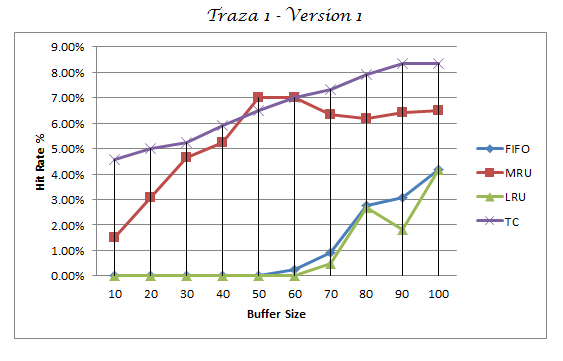
\includegraphics[height=11cm]{img/T1V1.png}
\end{center}  
\begin{center}
  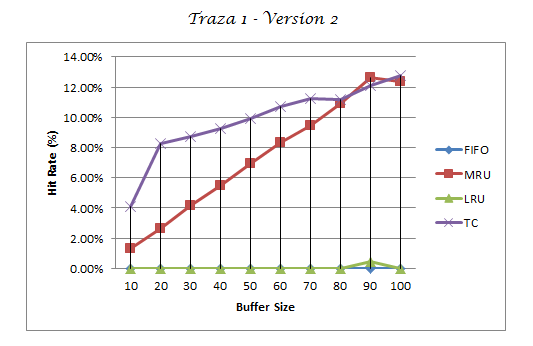
\includegraphics[height=11cm]{img/T1V2.png}
\end{center}  
\begin{center}  
  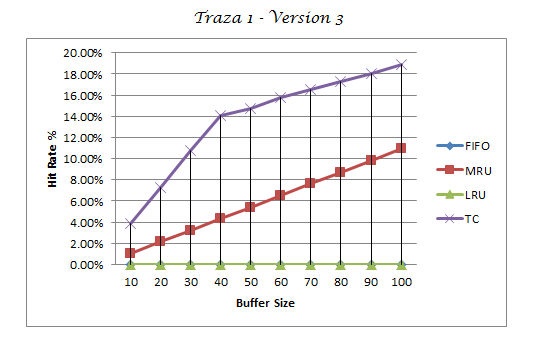
\includegraphics[height=11cm]{img/T1V3.png}
\end{center}  

\subsubsection*{Traza ``2''}
En esta traza lo que hacemos es generar un file scan sobre una tabla cualquiera, en la que se generan 1000 registros. Luego de esto se realiza una carga de registros de una tabla A, luego ocurre lo mismo con una tabla B en la que se reemplazaran en el buffer acordemente segun su tama\~no, finalmente hace una lectura de los registros de A, para luego hacer nuevamente una lectura sobre los registros de B. En la version 1, trabajamos con una cantidad de 50 registros al momento de cargar el buffer, en la 2 con una cantidad de 100 y en la 3 con una cantidad de 200. La escala Buffer Size representa el tama\'no del buffer
\begin{center}
  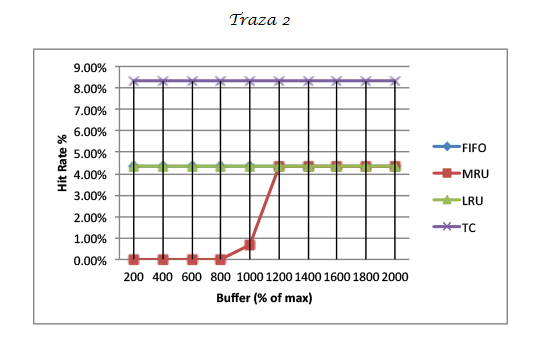
\includegraphics[height=11cm]{img/T2.png}
\end{center}  
\begin{center}
  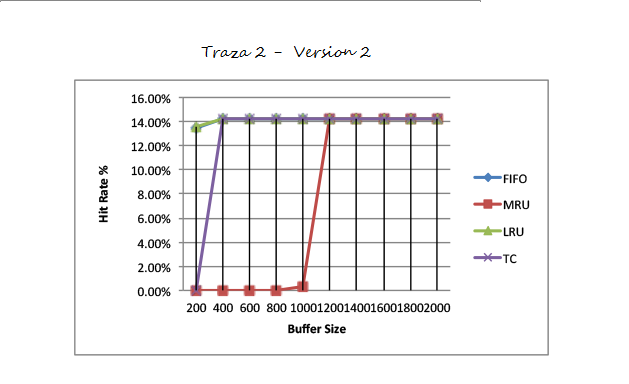
\includegraphics[height=11cm]{img/T2V2.png}
\end{center}  
\begin{center}
  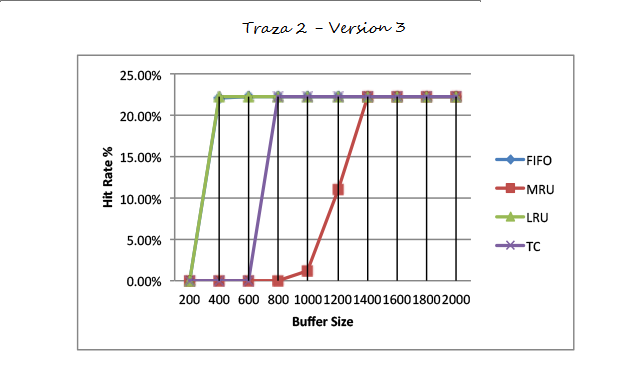
\includegraphics[height=11cm]{img/T2V3.png}
\end{center}  

\subsubsection*{Traza ``Block Nested Loops Join''}
En esta traza se hace un Block Nested Loops Join sobre dos tablas, se carga una tabla de a bloques y la segunda se carga despues de la carga de cada bloque de la primera, esto da la posibilidad de hits sobre los elementos de la segunda tabla. En la version 1, trabajamos con la versi\'on provista por la c\'atedra de SalesXProduct 250, la versi\'on 2 utiliza SalesXProduct 100. La escala Buffer Size representa el tama\'no del buffer
\begin{center}
  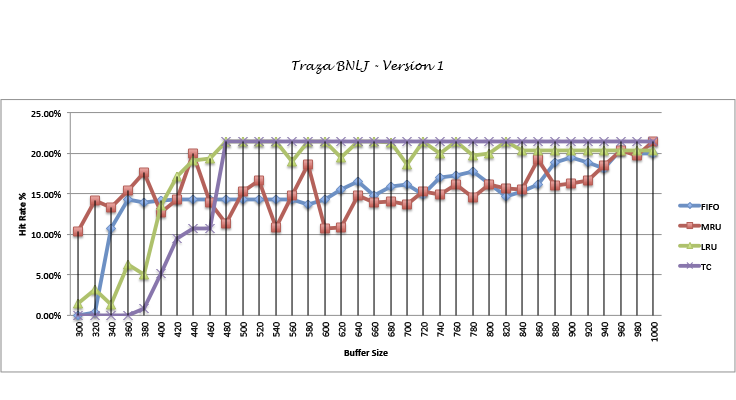
\includegraphics[scale=0.6]{img/T3V1.png}
\end{center}  
\begin{center}
  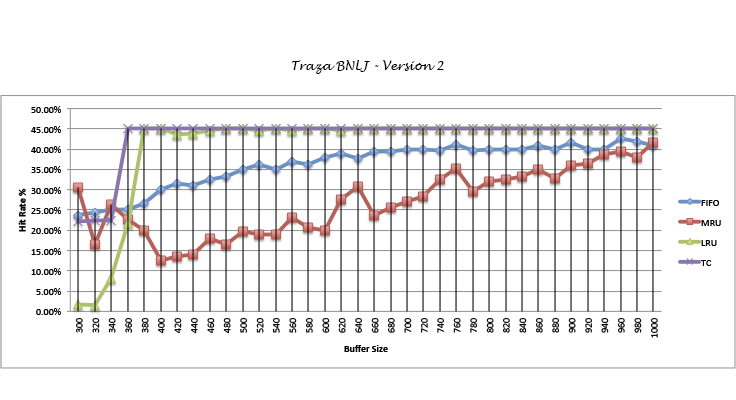
\includegraphics[scale=0.6]{img/T3V2.png}
\end{center}  


\subsection{An\'alisis de los resultados y conclusiones}

De estos resultados se observa un gran contraste entre las estrategias MRU y LRU. La traza 1 contiene un file scan en el medio de la misma, esto es muy malo para LRU y FIFO, puesto que descarta p\'aginas que luego van a volver a ser accedidas por otras que no lo ser\'an; por el contrario, es muy bueno para MRU, que simplemente descarta cada p\'agina apenas se almacena en memoria. Podemos ver que Touch Count se comporta incluso mejor que MRU en esta situaci\'on, las p\'aginas a las que se va a acceder varias veces se cargan en buffer al inicio de la ejecuci\'on, y la segunda lectura hace que pasen a la regi\'on caliente, por lo tanto, el file scan no las va a desalojar, dado que las p\'aginas del file scan entran en la regi\'on fr\'ia y son desalojadas de la misma. Por lo tanto, cuando se vuelve a acceder a las p\'aginas originales, \'estas siguen en la regi\'on caliente y por lo tanto dan hits.

Para la traza 2, el file scan se hace al principio de la ejecuci\'on; esto b\'asicamente vuelve completamente in\'util a la estrategia MRU, puesto que el buffer va a contener a todas las p\'aginas del file scan que entren durante toda la ejecuci\'on (es por esto que reci\'en se ve una cantidad de hits distinta de 0 cuando el buffer es m\'as grande que la cantidad de p\'aginas en la tabla sobre la que se hace file scan). Por el contrario, estrategias como FIFO y LRU no se ven afectadas, ya que simplemente las descartan r\'apidamente al llenarse el buffer. El comportamiento de Touch Count es interesante. Puesto que originalmente el buffer pool est\'a vac\'io, inevitablemente algunas de las p\'aginas del file scan van a quedar en la regi\'on caliente, a\'un sin haber recibido hits, y de ah\'i va a ser muy dif\'icil desalojarlas. Esto redunda en que el buffer efectivo es la mitad de tama\~no, por lo menos hasta que se produzcan hits que muevan dichas p\'aginas a la regi\'on caliente y por ende desalojen esas p\'aginas.

Para las trazas BNLJ, se observan resultados dispares, MRU tiene un funcionamiento que no var\'ia demasiado respecto del tama\'no del buffer, mientras que TC y LRU son en comparaci\'on peores con un buffer peque\'no, pero mucho mejores mientras m\'as grande es el buffer, en particular en la segunda versi\'on de la traza, LRU y TC alcanzan el pico r\'apidamente al crecer el buffer.

\subsection{Tabla de comparaciones}
En funci\'on de los an\'alisis anteriores se presenta la siguiente tabla comparativa de eficiencia de las distintas estrategias en los distintos contextos:
\begin{center}
\scalebox{0.7}{
  %\begin{tabular}{ | l | p{1.6cm} | p{1.6cm} | p{1.6cm} | p{1.6cm} | p{1.6cm} | p{1.6cm} |}
\begin{tabular}{ | l | c | c| c | c | c | c |}
    \hline
    \multirow{2}{*}{Algoritmo} & \multicolumn{2}{c|}{\textbf{Traza 1}} & \multicolumn{2}{c|}{\textbf{Traza 2}} & \multicolumn{2}{c|}{\textbf{BNLJ}} \\
    & Buffer Peque\~no & Buffer grande & Buffer Peque\~no & Buffer grande & Buffer Peque\~no & Buffer grande \\ \hline
    \textbf{Mejor Estrategia/s} & TC & TC & TC/LRU & TC & MRU & TC/LRU \\ \hline
    \textbf{Peor Estrategia/s} & LRU/FIFO & LRU/FIFO & MRU & --- & LRU & MRU \\ \hline
  \end{tabular}}
\end{center}

\\

Se puede ver que el algoritmo Touch Count casi siempre aparece como la mejor o una de las mejores estrategias para las diferentes trazas, existen condiciones en la que no es ideal, esto se debe a que al estar vac\'io y cargar p\'aginas \'estas pueden entrar en la regi\'on caliente sin haber recibido nunca hits, y por definici\'on misma del algoritmo es dif\'icil desalojar las p\'aginas de la regi\'on caliente, por lo tanto se desperdicia espacio del buffer en mantener p\'aginas que no van a dar hits. Esto podr\'ia ser remediado con un proceso que limpie cada la un per\'iodo de tiempo la regi\'on caliente, o por ejemplo que no haya regi\'on caliente hasta que no se produzca un hit, e ir extendiendo la regi\'on caliente hasta alcanzar la mitad a medida que se alcance la cantidad de buffers con hits.

Por otra parte, los algoritmos m\'as simples proporcionan una cantidad de hits a veces considerable, su problema es que todos tienen un caso particular en el que son muy malos, y eso en una base de datos en la que no se sabe con lo que se va a encontrar puede ser muy perjudicial y afectar el rendimiento al provocar muchos miss y sus consiguientes llamados a disco. Por el contrario, Touch Count es mucho m\'as dif\'icil encontrar un caso especial en el que se comporte mucho peor que los otros.

 

